\documentclass[main.tex]{subfiles}
\begin{document}

\subsection{Exercise 8}

For clarity, we denote with Greek indices those ranging from 1 to \(N\), the size of the vector of data; and with Latin indices those ranging from 1 to \(M\), the number of templates.

We are assuming that the data have a Gaussian distribution with a covariance matrix \(C\), and we are modelling their mean \(\mu_\alpha  \) as a sum of templates \(t_{i \alpha}\) with coefficients \(A_i\):
%
\begin{align}
\mu _\alpha = t_{i \alpha } A_i
\,,
\end{align}
%
where the Einstein summation convention has been used. 
Therefore, the likelihood is proportional to 
%
\begin{align}
\mathscr{L}(d_\alpha | A_i) \propto \exp(- \frac{1}{2} \qty(d_\alpha - A_{i} t_{i \alpha }) C^{-1}_{\alpha \beta } 
\qty(d_\beta - A_j t_{j \beta }))
\,.
\end{align}

The normalization only depends on the covariance matrix \(C_{\alpha \beta }\), which we assume is fixed.
Therefore, maximizing the likelihood\footnote{Which is equivalent to maximizing the posterior if we are using a flat prior.} is equivalent to minimizing the \(\chi^2\), which reads 
%
\begin{align}
\chi^2 = \qty(d_\alpha - A_{i} t_{i \alpha }) C^{-1}_{\alpha \beta } 
\qty(d_\beta - A_j t_{j \beta })
\,.
\end{align}

We want to minimize this as the amplitudes vary: therefore, we set the derivative with respect to \(A_k\) to zero,\footnote{The fact that the stationary point we will find is indeed a minimum can be checked by looking at the second derivative of \(\chi^2\): 
%
\begin{align}
\pdv[2]{\chi ^2}{A_k}{A_m} = 2 t_{k \alpha } C_{\alpha \beta }^{-1} t_{m \beta } 
\,,
\end{align}
%
and recalling that the inverse of the covariance matrix is positive definite.
}
%
\begin{align}
\pdv{\chi^2}{A_k} = -2 t_{k \alpha } C^{-1}_{\alpha \beta } \qty(d_\beta - A_j t_{j \beta }) = 0
\,,
\end{align}
%
which means that 
%
\begin{align}
t_{k \alpha } C^{-1}_{\alpha \beta } d_\beta = (t_{k \alpha } C^{-1}_{\alpha \beta }  t_{j \beta }) A_j
\,,
\end{align}
%
a linear system of \(M\) equations (indexed by \(k\)) in the \(M\) variables \(A_j\). 
If we denote the evaluations of bilinear forms in the data (\(N\)-dimensional) space with brackets, as \(a_\alpha C_{\alpha \beta } b_\beta \overset{\text{def}}{=} (a | C |b)\), this reads 
%
\begin{align}
(t | C^{-1} | d)_k &= (t | C^{-1} | t)_{kj} A_j  \\
\qty[(t | C^{-1} | t)^{-1}]_{mk} (t | C^{-1} | d)_k  &=
\underbrace{ \qty[(t | C^{-1} | t)^{-1}]_{mk}
(t | C^{-1} | t)_{kj}}_{= \delta_{mj}} A_j = A_m  \\
A_m &= \qty[(t | C^{-1} | t)^{-1}]_{mk} (t | C^{-1} | d)_k
\,, \label{eq:template-fitting}
\end{align}
%
where the inverse of \((t | C^{-1} | t)\) is to be computed in the \(M\)-dimensional vector space. 

\subsection{Exercise 9}

Our model for the mean value is in the form \(\mu (\Theta , A) = A \overline{x}(\Theta )\), where \(\overline{x}\) is a generic function of \(\Theta \), while \(A\) is our scale parameter.\footnote{This is not specified in the problem, but it seems natural to think that \(\abs{\overline{x}(\Theta )}\) is a constant for varying \(\Theta \). } 
Our likelihood then reads 
%
\begin{align}
\mathscr{L}(x | \Theta , A) = \underbrace{\frac{1}{(2\pi )^{N/2} \sqrt{\det C}}}_{B_1 }
\exp(- \frac{1}{2} (x - A \overline{x}(\Theta ))^{\top} C^{-1} (x- A \overline{x}(\Theta )))
\,.
\end{align}

If the priors for both \(A\) and \(\Theta \) are flat, this corresponds to the joint posterior \(P (\Theta , A | x)\). 
We want to marginalize over \(A\), which amounts to integrating over it: dropping the dependence on \(\Theta \) of \(\overline{x}\) and defining \(V = C^{-1}\) we find
%
\begin{align}
P(\Theta | x) 
&= B_1  \int \exp(- \frac{1}{2} (x - A \overline{x})^{\top} V (x- A \overline{x})) \dd{A}  \\
&= B_1  \int \exp(- \frac{1}{2} \qty(x^{\top} V x -2 A \overline{x}^{\top} V x + A^2 \overline{x}^{\top} V \overline{x})) \dd{A} 
\marginnote{Used the symmetry of \(V\).}
\,.
\end{align}

The amplitude being negative makes little sense in a typical physical context, however the Gaussian integral can be done analytically only over the whole of \(\mathbb{R}\).

In order to get analytical results, here we will marginalize by integrating over negative amplitudes as well (\(A \in \mathbb{R}\)); the last figure (\ref{fig:marginalization}) will show how only integrating over positive amplitudes only would have looked (by numerical calculation) in a simple case.
In general if one wishes to perform the integral over \(A \in (0, + \infty )\) the tabulated values of the error function may be used.

Applying the formula for the single-variable Gaussian integral \eqref{eq:single-variable-gaussian-integral} (the bilinear forms are all evaluated to yield scalars, we are only integrating over the scalar \(A\)!) we then get 
%
\begin{align}
P(\Theta | x) &= \underbrace{B_1  \exp(- \frac{1}{2} x^{\top} V x )}_{B_2 } 
\exp( \frac{1}{2} \frac{(\overline{x}^{\top} V x)^2}{(\overline{x}^{\top} V \overline{x})}) 
\sqrt{ \frac{2 \pi }{\overline{x}^{\top} V \overline{x}}}  \\
&= B_2 \sqrt{\frac{2 \pi}{\overline{x}^{\top}V \overline{x}}}
\exp( \frac{1}{2} \frac{\overline{x}^{\top} \Omega \overline{x}}{\overline{x}^{\top}V \overline{x}})
\,,
\end{align}
%
where we defined the bilinear form \(\Omega = V x x^{\top} V^{\top}\).\footnote{With explicit indices, \(\Omega_{im} = V_{ij} x_j x_k V_{km}\).}

% We can observe that all information about the scale of \(\overline{x}\) has been lost: if we map \(\overline{x} \to A \overline{x}\) the argument of the exponential does not change, therefore the only change comes from the factor in front, and the posterior \(P\) is mapped to \(P / A\). 

\subsubsection{An application of posterior marginalization in this fashion}

Let us consider a simple example of this as a sanity check: suppose that \(x\) is two-dimensional, and \(\overline{x}(\Theta ) = (\cos \Theta , \sin \Theta )^{\top}\); further, suppose that \(V\) is diagonal, so that 
%
\begin{align}
V = \left[\begin{array}{cc}
\sigma_x^{-2} & 0 \\ 
0 & \sigma _y^{-2}
\end{array}\right]
\,.
\end{align}

Also, suppose that the observed data parameter is 
%
\begin{align}
x = A_x \left[\begin{array}{c}
\cos \varphi  \\ 
\sin \varphi 
\end{array}\right]
\,.
\end{align}

Then, the multiplicative constant in front of the marginalized posterior reads 
%
\begin{align}
B_2 = B_1 \exp(- \frac{1}{2} A_x^2 \qty( \frac{\cos^2\varphi}{\sigma^2_x} + \frac{\sin^2\varphi}{\sigma^2_y}))
\,;
\end{align}
%
while the bilinear form \(\Omega \) is 
%
\begin{align}
\Omega &= A_x^2
\left[\begin{array}{cc}
\sigma_x^{-2} & 0 \\ 
0 & \sigma _y^{-2}
\end{array}\right]
\left[\begin{array}{cc}
\cos^2 \varphi  & \cos \varphi \sin \varphi  \\ 
\cos \varphi \sin \varphi  & \sin^2 \varphi 
\end{array}\right]
\left[\begin{array}{cc}
\sigma_x^{-2} & 0 \\ 
0 & \sigma _y^{-2}
\end{array}\right]  \\
&= A_x^2\left[\begin{array}{cc}
\cos^2 \varphi / \sigma_x^{4} & \cos \varphi \sin \varphi / \sigma_x^2 \sigma _y^2 \\ 
\cos \varphi \sin \varphi / \sigma_x^2 \sigma _y^2 & \sin^2 \varphi / \sigma_y^{4}
\end{array}\right]
\,.
\end{align}

Then, when we  evaluate the marginalized posterior we will find something in the form
%
\begin{align}
P(\Theta | x) &= B_1 \sqrt{2 \pi } \qty( \frac{\cos^2\Theta }{\sigma_x^2} + \frac{\sin^2 \Theta }{\sigma _y^2})^{-1/2}
\exp( A_x^2 F(\Theta , \varphi ))
\,,
\end{align}
%
where \(F (\Theta , \varphi )\) is some function whose specific form does not really matter.\footnote{For completeness, here is the full expression: 
%
\begin{align}
\begin{split}
F(\Theta , \varphi ) &=
- \frac{1}{2} \qty( \frac{\cos^2\varphi}{\sigma^2_x} + \frac{\sin^2\varphi}{\sigma^2_y})+  \\
&\phantom{=}\ 
+ 
\qty( \frac{\cos^2 \Theta}{\sigma _x^2} + \frac{\sin^2 \Theta }{\sigma _y^2})^{-1}
\qty[ 
    \frac{\cos^2 \Theta \cos^2 \varphi }{\sigma _x^{4}}
    +2\frac{\cos \Theta \sin \Theta \cos \varphi \sin \varphi  }{\sigma _x^{2} \sigma _y^{2}}
    +\frac{\sin^2 \Theta \sin^2 \varphi }{\sigma _y^{4}}
]
\,.
\end{split}
\end{align}
%
}

The amplitude of the observed data vector, \(A_x\), appears in a rather simple way, as a multiplicative prefactor in the exponent: it can affect the shape of the distribution, but not its mean.
Specifically, we can see that scaling \(A_x\) is equivalent to scaling \(\sigma _x\) and \(\sigma _y\) simultaneously in the opposite direction --- this is rather intuitive, since the angular size of the distribution as seen from the origin is smaller if it is further away. 

% Therefore, we see that by marginalizing over \(A\) we have ``forgotten'' any scaling information about \(x\). 

\begin{figure}[ht]
\centering
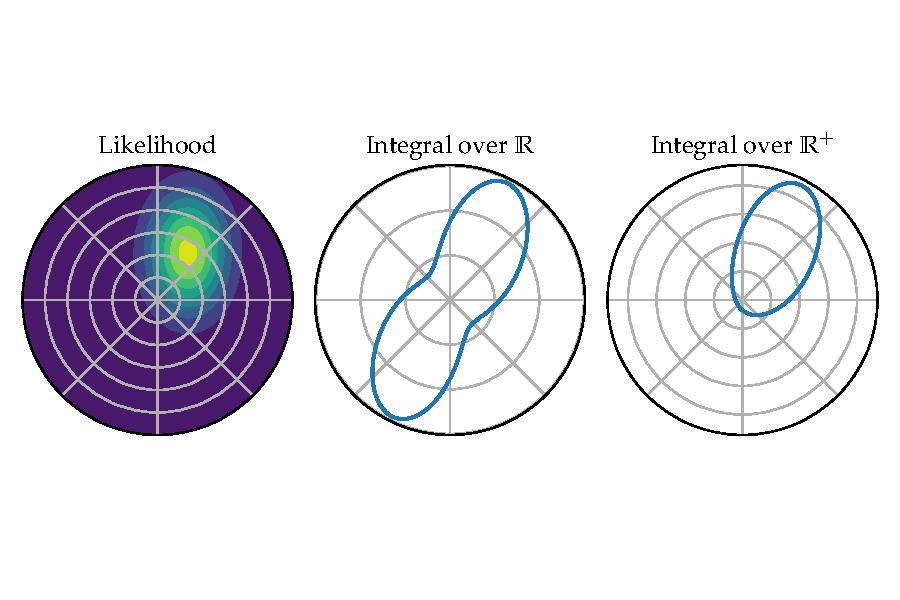
\includegraphics[width=\textwidth]{figures/marginalization.pdf}
\caption{Marginalization: the left plot shows the full likelihood in terms of \(A\) and \(\Theta \); the middle plot shows the result of marginalization as shown in the previous calculation (the posterior as a function of \(\Theta \)); the right plot shows the result of the more physically meaningful marginalization over \(A \in (0, + \infty )\) only.
Here the likelihood is a diagonal Gaussian with \(\sigma _x = \num{1.2}\) and \(\sigma _y = \num{1.8}\), centered in \(A_x = \num{2.5}\) and \(\varphi = \SI{1}{rad}\).}
\label{fig:marginalization}
\end{figure}

\subsubsection{Likelihood marginalization}

So far we have considered the posterior \(P(\Theta | x)\), the marginalized posterior, a function of the parameter(s) \(\Theta \); however we may also be interested in the marginalized likelihood \(\mathscr{L}(x | \Theta )\), whose expression is the same as the one we found for \(P(\Theta | x)\).
Let us write it in a way which makes the dependence on \(x\) more explicit: 
%
\begin{align} \label{eq:marginalized-likelihood}
\mathscr{L}(x | \Theta ) = \underbrace{B_1 \sqrt{\frac{2 \pi }{\overline{x}^{\top} V \overline{x}}}}_{B_3 } \exp(- \frac{1}{2} x^{\top} V x + 
\frac{1}{2}
\frac{(\overline{x}^{\top} V x)^2}{\overline{x}^{\top} V \overline{x}})
\,,
\end{align}
%
which can be simplified by making use of the fact that the best-fit template amplitude we found in the last exercise (equation \eqref{eq:template-fitting}) can be applied here, with the single template \(t = \overline{x}\), the single amplitude \(A\), the data \(d = x\), and the inverse covariance matrix \(C^{-1}= V\): the fitting value for \(A \) is 
%
\begin{align}
\hat{A} = \frac{\overline{x}^{\top} V x}{\overline{x}^{\top} V \overline{x}}
\,;
\end{align}
%
therefore the likelihood is 
%
\begin{align}
\mathscr{L}(x | \Theta ) = B_3 \exp(- \frac{1}{2} x^{\top} V x +
\frac{1}{2}
 \hat{A} \overline{x}^{\top} V x)
\,.
\end{align}

This can be rewritten in the canonical MVN form by making use of the matrix square completion formula \eqref{eq:square-completion}, with \(A = -V\) and \(\vec{b}^{\top} = \hat{A} \overline{x}^{\top} V\): 
%
\begin{align}
\begin{split}
- \frac{1}{2} x^{\top} V x + \frac{1}{2} \hat{A} \overline{x}^{\top} V x
&= - \frac{1}{2} 
\qty(x - \frac{1}{2} V^{-1} \hat{A} (\overline{x}^{\top} V)^{\top})^{\top} V
\qty(x - \frac{1}{2} V^{-1} \hat{A} (\overline{x}^{\top} V)^{\top}) \\
&\phantom{=}\ 
+ \frac{1}{8} \hat{A}^2 (\overline{x}^{\top} V) V^{-1} (\overline{x}^{\top} V)^{\top}  
\end{split}\\
&= - \frac{1}{2} 
\qty(x - \frac{1}{2} \hat{A} \overline{x})^{\top}
V 
\qty(x - \frac{1}{2} \hat{A} \overline{x})
+ 
\frac{1}{8} \hat{A}^2 \overline{x}^{\top} V \overline{x}
\,.
\end{align}

Therefore, the marginalized likelihood reads 
%
\begin{align}
\mathscr{L}(x | \Theta ) = B_3 \exp( \frac{1}{8} \hat{A}^2 \overline{x}^{\top} V \overline{x}) \exp(- \frac{1}{2} \qty(x - \frac{1}{2} \hat{A} \overline{x})^{\top} V \qty( \frac{1}{2} x - \hat{A} \overline{x}))
\,.
\end{align}

We must be careful with this expression: it looks like a multivariate normal in \(\overline{x}\), however \(\hat{A}\) is not in general independent of it.
If neither the estimate for \(\hat{A}\) nor the expression \(\overline{x}^{\top} V \overline{x}\) vary significantly in the range of \(\overline{x}\) we are interested in, then we can consider this expression for the likelihood as Gaussian in \(x\), or as a marginalized posterior which is Gaussian in \(\overline{x}\).

% A clearer way to see that this is indeed still a MVN is to come back to the original expression \eqref{eq:marginalized-likelihood}, and to write it as 
% %
% \begin{align}
% \mathscr{L} (x | \Theta ) = B_3 \exp(- \frac{1}{2} x^{\top} \qty(V - \frac{V \overline{x} \overline{x}^{\top} V}{\overline{x}^{\top} V \overline{x}}) x )
% \,,
% \end{align}
% %
% thus showing that the likelihood is a \emph{zero-mean} MVN with covariance given by 
% %
% \begin{align}
% \qty[V - \frac{V \overline{x} \overline{x}^{\top} V}{\overline{x}^{\top} V \overline{x}}]^{-1}
% \,.
% \end{align}


\end{document}
